\section{Minimum phase systems}

\begin{definition}[\textit{Minimum phase system}]
    A system is classified as a minimum phase system if all the zeros of its transfer function lie inside the unit circle in the complex plane.
\end{definition}
When considering a step input signal at a certain time instant, the response of a minimum phase system typically exhibits a behavior where the output initially moves towards its final value. 
This behavior is due to the absence of zeros outside the unit circle, which results in a stable and predictable response.

Conversely, in the case of a non-minimum phase system, some zeros of the transfer function lie outside the unit circle. 
As a consequence, the initial response of the system may move in the opposite direction compared to its final value. 
This behavior arises due to the presence of unstable or oscillatory modes introduced by the zeros outside the unit circle.

Consider a step on the input signal at a certain time instant: 
\begin{figure}[H]
    \centering
    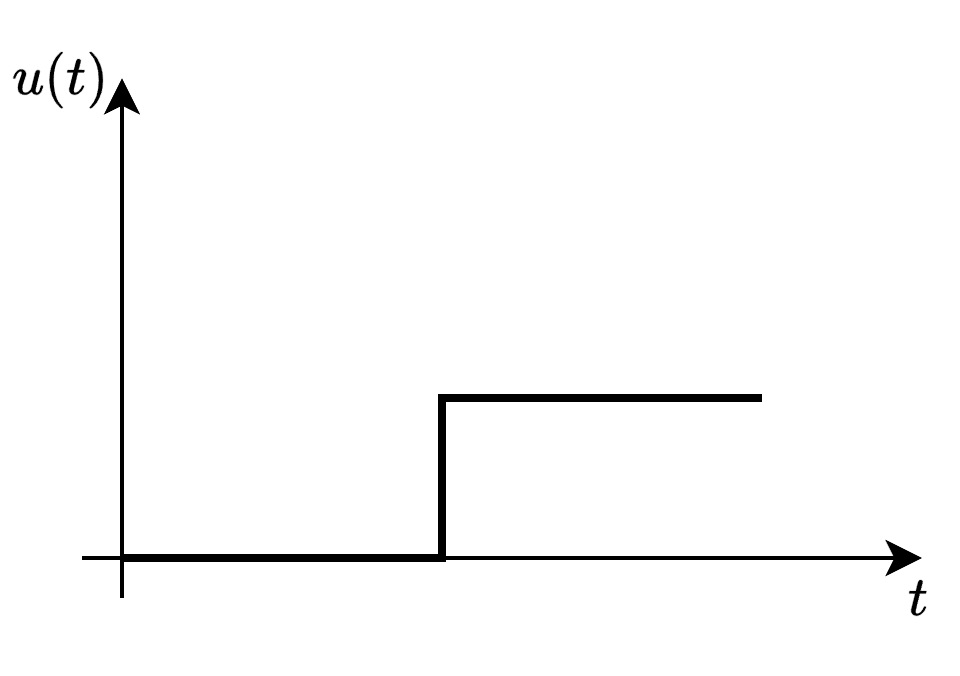
\includegraphics[width=0.4\linewidth]{images/phase.png}
\end{figure}
Visually, this difference in behavior between minimum and non-minimum phase systems can be illustrated by observing the direction of the initial response relative to the final value in the step response plot. 
In minimum phase systems, the initial response moves towards the final value, while in non-minimum phase systems, it may initially move away from the final value before eventually converging to it.
\begin{figure}[H]
    \centering
    \begin{subfigure}{0.49\textwidth}
        \centering
        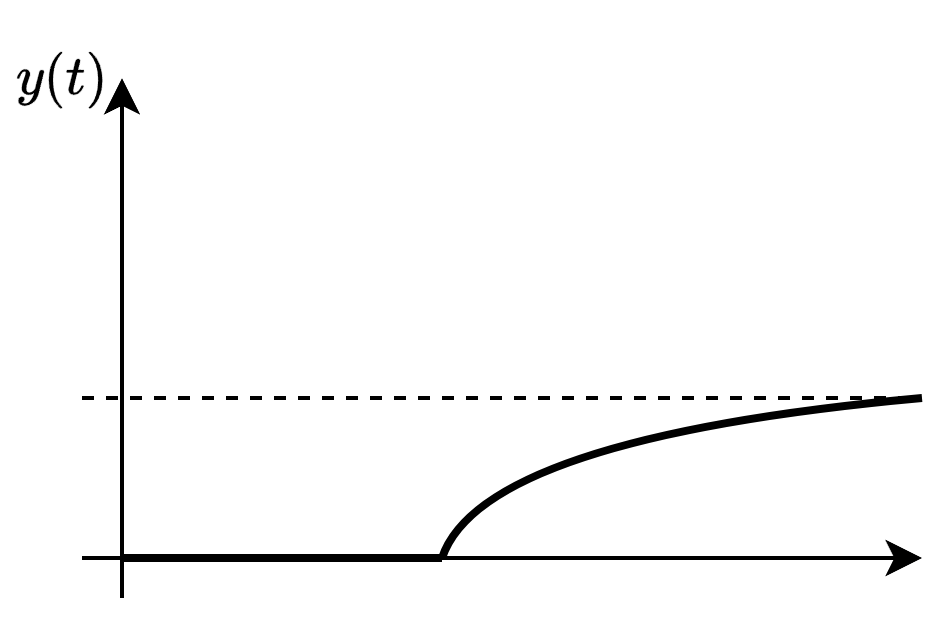
\includegraphics[width=0.75\linewidth]{images/phase1.png} 
        \caption{Minimum phase system}
    \end{subfigure}
    \begin{subfigure}{0.49\textwidth}
        \centering
        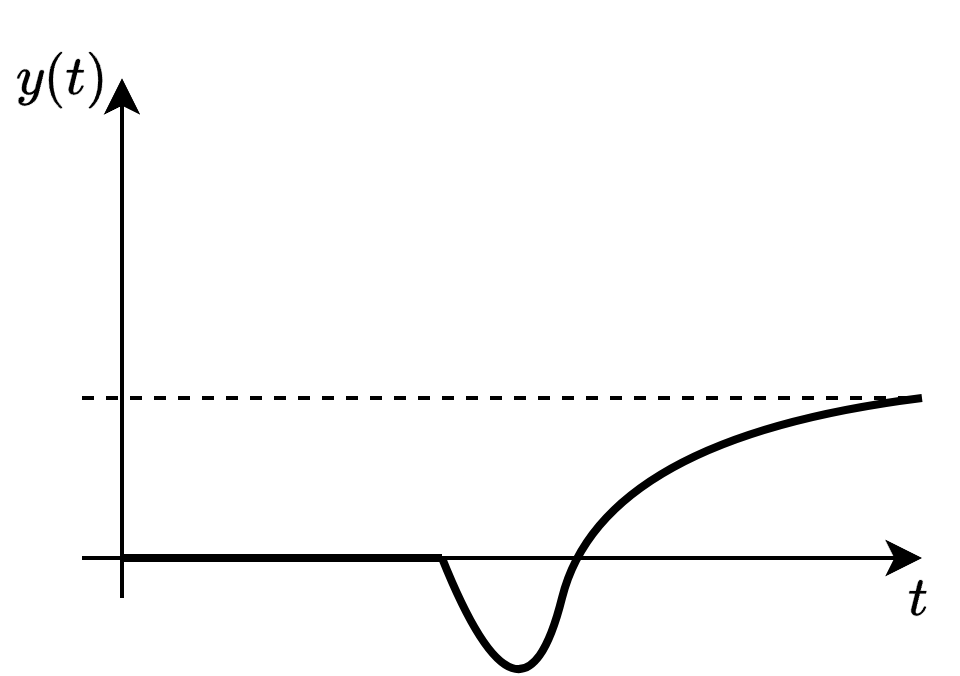
\includegraphics[width=0.75\linewidth]{images/phase2.png}
        \caption{Non-minimum phase system}
    \end{subfigure}
    \caption{System comparison}
\end{figure}